% Preambel mit Einstellungen importieren
% Document type and used packages
\documentclass[open=right, % Sorgt für Umbruch bei Chapter (any erzeugt keine Leerseiten) -> Kapitel darf nur auf der rechten Seite beginnen
    paper=A4,               % DIN-A4-Papier
    a4paper,                % DIN-A4-Papier
    12pt,                   % Schriftgöße
    headings=small,         % Kleine Überschriften
    headsepline=true,       % Trennlinie am Kopf der Seite
    footsepline=false,      % Keine Trennlinie am Fuß der Seite
    bibliography=totoc,     % Literaturverzeichnis in das Inhaltsverzeichnis aufnehmen
    twoside=on,             % Doppelseitiger Druck - auf off stellen für einseitig
    DIV=7,                  % Verhältnis der Ränder zum bedruckten Bereich
    chapterprefix=false,     % Kapitel x vor dem Kapitelnamen
    cleardoublepage=plain]{scrbook}


\usepackage{morewrites}

% Pakete einbinden, die benötigt werden
\usepackage{scrpage2}
\usepackage[utf8]{inputenc}       % Dateien in UTF-8 benutzen
\usepackage[T1]{fontenc}          % Zeichenkodierung
\usepackage{graphicx}             % Bilder einbinden
\usepackage[main=ngerman, english]{babel}       % Deutsch und Englisch unterstützen
\usepackage{xcolor}               % Color support
\usepackage{amsmath}              % Matheamtische Formeln
\usepackage{amsfonts}             % Mathematische Zeichensätze
\usepackage{amssymb}              % Mathematische Symbole
\usepackage{float}                % Fließende Objekte (Tabellen, Grafiken etc.)
\usepackage{booktabs}             % Korrekter Tabellensatz
\usepackage[printonlyused, withpage, footnote]{acronym}  % Abkürzungsverzeichnis [nur verwendete Abkürzugen]
\usepackage{makeidx}              % Sachregister
\usepackage{listings}             % Source Code listings
\usepackage{listingsutf8}         % Listings in UTF8
\usepackage[hang,font={sf,footnotesize},labelfont={footnotesize,bf}]{caption} % Beschriftungen
\usepackage[scaled]{helvet}       % Schrift Helvetia laden
\usepackage[absolute]{textpos}	  % Absolute Textpositionen (für Deckblatt)
\usepackage{calc}                 % Berechnung von Positionen
\usepackage{blindtext}            % Blindtexte
\usepackage[bottom=40mm,left=35mm,right=35mm,top=30mm]{geometry} % Ränder ändern
\usepackage{setspace}             % Abstände korrigieren
\usepackage{ifthen}               % Logische Bedingungen mit ifthenelse
\usepackage{scrhack}              % Get rid of tocbasic warnings
\usepackage[pagebackref=false,german]{hyperref}  % Hyperlinks
\usepackage[all]{hypcap}          % Korrekte Verlinkung von Floats
\usepackage[autostyle=true,german=quotes]{csquotes}   % Zitate
\usepackage[backend=biber,
  isbn=true,                     % ISBN nicht anzeigen, gleiches geht mit nahezu allen anderen Feldern
  sortlocale=de_DE,               % Sortierung der Einträge für Deutsch
  %sortlocale=en_US,              % Sortierung der Einträge für Englisch
  autocite=inline,                % regelt Aussehen für \autocite (inline=\parancite)
  hyperref=true,                  % Hyperlinks für Ziate
  %style=ieee                     % Zitate als Zahlen [1]
  %style=alphabetic               % Zitate als Kürzel und Jahr [Ein05]
  %style=authoryear                % Zitate Author und Jahr [Einstein (1905)]
  style=LNI
]{biblatex}                       % Literaturverwaltung mit BibLaTeX
\usepackage{rotating}             % Seiten drehen
\usepackage{harveyballs}          % Harveyballs
\usepackage{tcolorbox}
\usepackage[export]{adjustbox}
\usepackage{subcaption}
\usepackage{color}
\usepackage{colortbl}
\usepackage{wrapfig}
\usepackage{todonotes}
\usepackage{tabularx}
\newcolumntype{b}{>{\hsize=1.2\hsize}X}
\newcolumntype{m}{>{\hsize=.5\hsize}X}
\newcolumntype{s}{>{\hsize=.3\hsize}X}
\usepackage{tikz}


\setlength{\bibitemsep}{1em}     % Abstand zwischen den Literaturangaben
\setlength{\bibhang}{2em}        % Einzug nach jeweils erster Zeile

% Trennung von URLs im Literaturverzeichnis (große Werte [> 10000] verhindern die Trennung)
\defcounter{biburlnumpenalty}{10} % Strafe für Trennung in URL nach Zahl
\defcounter{biburlucpenalty}{500}  % Strafe für Trennung in URL nach Großbuchstaben
\defcounter{biburllcpenalty}{500}  % Strafe für Trennung in URL nach Kleinbuchstaben

% Farben definieren
\definecolor{linkblue}{RGB}{0, 0, 100}
\definecolor{linkblack}{RGB}{0, 0, 0}
\definecolor{comment}{RGB}{63, 127, 95}
\definecolor{darkgreen}{RGB}{14, 144, 102}
\definecolor{darkblue}{RGB}{0,0,168}
\definecolor{darkred}{RGB}{128,0,0}
\definecolor{javadoccomment}{RGB}{0,0,240}
\definecolor{Gray}{RGB}{242,242,242}

% Einstellungen für das Hyperlink-Paket
\hypersetup{
    colorlinks=true,      % Farbige links verwenden
%    allcolors=linkblue,
    linktoc=all,          % Links im Inhaltsverzeichnis
    linkcolor=linkblack,  % Querverweise
    citecolor=linkblack,  % Literaturangaben
	filecolor=linkblack,  % Dateilinks
	urlcolor=linkblack    % URLs
}

% Einstellungen für Quelltexte
\definecolor{backcolour}{rgb}{0.95,0.95,0.92}
\definecolor{codegray}{rgb}{0.5,0.5,0.5}
\lstset{
      xleftmargin=0.1cm,
      basicstyle=\footnotesize\ttfamily,
      keywordstyle=\color{darkgreen},
      identifierstyle=\color{darkblue},
      commentstyle=\color{comment},
      stringstyle=\color{darkred},
      tabsize=2,
      lineskip={2pt},
      columns=flexible,
      inputencoding=utf8,
      captionpos=b,
      backgroundcolor=\color{backcolour},   
      breakautoindent=true,
	  breakindent=2em,
	  breaklines=true,
	  prebreak=,
	  postbreak=,
      numbers=left,                    
      numbersep=5pt,  
      numberstyle=\tiny\color{codegray},  
      showspaces=false,      % Keine Leerzeichensymbole
      showtabs=false,        % Keine Tabsymbole
      showstringspaces=false,% Leerzeichen in Strings
      morecomment=[s][\color{javadoccomment}]{/**}{*/},
      literate={Ö}{{\"O}}1 {Ä}{{\"A}}1 {Ü}{{\"U}}1 {ß}{{\ss}}2 {ü}{{\"u}}1 {ä}{{\"a}}1 {ö}{{\"o}}1
}


\urlstyle{same}

% Einstellungen für Überschriften
\renewcommand*{\chapterformat}{%
  \Large~\thechapter. ~   		% Große Schrift
  \vspace{0.3cm}               	% Abstand zum Titel des Kapitels
}

% Abstände für die Überschriften setzen
\renewcommand{\chapterheadstartvskip}{\vspace*{2.6cm}}
\renewcommand{\chapterheadendvskip}{\vspace*{1.5cm}}

\RedeclareSectionCommand[
  beforeskip=-1.8\baselineskip,
  afterskip=0.25\baselineskip]{section}

\RedeclareSectionCommand[
  beforeskip=-1.8\baselineskip,
  afterskip=0.15\baselineskip]{subsection}

\RedeclareSectionCommand[
  beforeskip=-1.8\baselineskip,
  afterskip=0.15\baselineskip]{subsubsection}


% In der Kopfzeile nur die kurze Kapitelbezeichnung (ohne Kapitel davor)
\renewcommand*\chaptermarkformat{\thechapter\autodot\enskip}
\automark[chapter]{chapter}

% Einstellungen für Schriftarten
\setkomafont{pagehead}{\normalfont\sffamily}
\setkomafont{pagenumber}{\normalfont\sffamily}
\setkomafont{paragraph}{\sffamily\bfseries\small}
\setkomafont{subsubsection}{\sffamily\itshape\bfseries\small}
\addtokomafont{footnote}{\footnotesize}
\setkomafont{chapter}{\LARGE\selectfont\bfseries}

% Wichtige Abstände
\setlength{\parskip}{0.2cm}  % 2mm Abstand zwischen zwei Absätzen
\setlength{\parindent}{0mm}  % Absätze nicht einziehen
\clubpenalty = 10000         % Keine "Schusterjungen"
\widowpenalty = 10000        % Keine "Hurenkinder"
\displaywidowpenalty = 10000 % Keine "Hurenkinder"
\renewcommand{\footnotesize}{\fontsize{9}{10}\selectfont} % Größe der Fußnoten
\setlength{\footnotesep}{8pt} % Abstand zwischen den Fußnoten

% Index erzeugen
\makeindex

% Einfacher Font-Wechsel über dieses Makro
\newcommand{\changefont}[3]{
\fontfamily{#1} \fontseries{#2} \fontshape{#3} \selectfont}

% Eigenes Makro für Bilder
\newcommand{\bild}[3]{
\begin{figure}[h]
  \centering
  \includegraphics[width=#2]{#1}
  \caption{#3}
  \label{#1}
\end{figure}}

% Wo liegt Sourcecode?
\newcommand{\srcloc}{src/}

% Wo sind die Bilder?
\graphicspath{{bilder/}}

% Makros für typographisch korrekte Abkürzungen
\newcommand{\zb}[0]{z.\,B.\ }
\newcommand{\dahe}[0]{d.\,h.\ }
\newcommand{\ua}[0]{u.\,a.\ }

% Flags für Veröffentlichung und Sperrvermerk
\newboolean{hsmapublizieren}
\newboolean{hsmasperrvermerk}


% Dokumenteninfos importieren
% In docinfo.tex sind Titel, Autor, Abstract zu definieren
% -------------------------------------------------------
% Daten für die Arbeit
% Wenn hier alles korrekt eingetragen wurde, wird das Titelblatt
% automatisch generiert. D.h. die Datei titelblatt.tex muss nicht mehr
% angepasst werden.

\newcommand{\hsmasprache}{de} % de oder en für Deutsch oder Englisch
% Für korrekt sortierte Literatureinträge, noch preambel.tex anpassen
% und zwar bei \usepackage[main=ngerman, english]{babel},
% \usepackage[pagebackref=false,german]{hyperref}
% und \usepackage[autostyle=true,german=quotes]{csquotes}

% Titel der Arbeit auf Deutsch
\newcommand{\hsmatitelde}{Aufgabenfokussierung auf Autoencoder und automatisches Transferlernen}

% Titel der Arbeit auf Englisch
\newcommand{\hsmatitelen}{Task focusing on autoencoder and automatic transfer learning}

% Weitere Informationen zur Arbeit
\newcommand{\hsmaort}{Offenburg}    % Ort
\newcommand{\hsmaautorvname}{Sebastian} % Vorname(n)
\newcommand{\hsmaautornname}{Hoch} % Nachname(n)
\newcommand{\hsmadatum}{30 Juni 2020} % Datum der Abgabe
\newcommand{\hsmajahr}{2020} % Jahr der Abgabe
\newcommand{\hsmafirma}{PSIORI GmbH} % Firma bei der die Arbeit durchgeführt wurde
\newcommand{\hsmabetreuer}{Prof. Dr.-Ing. Janis Keuper, Hochschule Offenburg} % Betreuer an der Hochschule
\newcommand{\hsmazweitkorrektor}{Dr. rer. nat. Sascha Lange, PSIORI GmbH} % Betreuer im Unternehmen oder Zweitkorrektor
\newcommand{\hsmafakultaet}{EMI} % Fakultät
\newcommand{\hsmastudiengang}{INFM} % Studiengangsabkürzung. 
% Diese wird in titelblatt.tex definiert. Bisher AI, EI, MK und INFM. Bitte ergänzen.

% Zustimmung zur Veröffentlichung
\setboolean{hsmapublizieren}{true}   
\setboolean{hsmasperrvermerk}{false} 

% -------------------------------------------------------
% Abstract

% Kurze (maximal halbseitige) Beschreibung, worum es in der Arbeit geht auf Deutsch
\newcommand{\hsmaabstractde}{
	
	Im Rahmen dieser Arbeit wurden drei Werkzeuge erstellt, um Merkmalextraktion, Transferlernen und AutoMl zu kombinieren.
	Das erste Werkzeug gleicht eine Schwäche eines Autoencoders aus. Beim Training eines Autoencoders wird die Rekonstruktion, also der Output des Modelles und nicht direkt die Einbettung als Bewertungskriterium herangezogen. Um diese Schwäche zu kompensieren, wurde der SCAE erstellt. Dieses Werkzeug ist ein Autoencoder mit weiterem Ausgang. Die Datenrepräsentation wird durch ein zweites Kriterium gestärkt. Das zweite Werkzeug nutzt die Datenrepräsentation, um eine Aufgabe mittels Transferlernen durchzuführen. Das zweite Kriterium wird durch ein neues Kriterium ersetzt. Als drittes Werkzeug wurde der TCSCAE um Funktionen des AutoMl erweitert. Die besten Hyperparameter werden automatisch gefunden. Die Werkzeuge wurden anhand von echten Datensätzen getestet und validiert. Dabei hat sich gezeigt, dass mit den Werkzeugen eine ähnlich gute Leistung wie auf dem herkömmlichen Weg erreicht werden kann und das durch das Transferlern sogar aufwand reduziert werden kann.
	\todo{Abstract neu schreiben}
	Beschreibugn der Tools weniger konkret?
}


% Kurze (maximal halbseitige) Beschreibung, worum es in der Arbeit geht auf Englisch

\newcommand{\hsmaabstracten}{Englische Version von Lorem ipsum dolor sit amet, consetetur sadipscing elitr, sed diam nonumy eirmod tempor invidunt ut labore et dolore magna aliquyam erat, sed diam voluptua. At vero eos et accusam et justo duo dolores et ea rebum. Stet clita kasd gubergren, no sea takimata sanctus est Lorem ipsum dolor sit amet. Lorem ipsum dolor sit amet, consetetur sadipscing elitr, sed diam nonumy eirmod tempor invidunt ut labore et dolore magna aliquyam erat, sed diam voluptua. At vero eos et accusam et justo duo dolores et ea rebum. Stet clita kasd gubergren, no sea takimata sanctus est Lorem ipsum dolor sit amet.
\todo{Abstract ins Englische übersetzen}}


% Literatur-Datenbank
\addbibresource{literatur.bib}   % BibLaTeX-Datei mit Literaturquellen einbinden

\begin{document}
\frontmatter

% Römische Ziffern für die "Front-Matter"
\setcounter{page}{0}
\changefont{ptm}{m}{n}  % Times New Roman für den Fließtext
\renewcommand{\rmdefault}{ptm}

% Titelblatt
% -------------------------------------------------------
% In dieser Datei sollten eigentlich keine Veränderungen mehr
% notwendig sein.
% -------------------------------------------------------

\thispagestyle{empty}

% Fakultät
% -------------------------------------------------------
\ifthenelse{\equal{\hsmafakultaet}{EI}}%
  {\newcommand{\hsmafakultaetlangde}{Fakultät Elektrotechnik und Informationstechnik}%
   \newcommand{\hsmafakultaetlangen}{Department of Electrical Engineering and Computer Science}}{}
\ifthenelse{\equal{\hsmafakultaet}{EMI}}%
{\newcommand{\hsmafakultaetlangde}{Fakultät Elektrotechnik, Medizintechnik und Informatik}%
	\newcommand{\hsmafakultaetlangen}{Department of Electrical Engineering, Medical Engineering and Computer Science}}{}



\ifthenelse{\equal{\hsmastudiengang}{AI}}%
{\newcommand{\hsmastudienganglangde}{Angewandte Informatik}%
	\newcommand{\hsmastudienganglangen}{Applied Computer Science}%
	\newcommand{\hsmatypde}{BACHELORARBEIT}%
	\newcommand{\hsmatypen}{BACHELOR THESIS}%
	\newcommand{\hsmagrad}{\hsmabachelor}}{}

\ifthenelse{\equal{\hsmastudiengang}{EI}}%
{\newcommand{\hsmastudienganglangde}{Elektrotechnik/Informationstechnik}%
	\newcommand{\hsmastudienganglangen}{Electrical Engineering/Information Technology}%
	\newcommand{\hsmatypde}{BACHELORARBEIT}%
	\newcommand{\hsmatypen}{BACHELOR THESIS}%
	\newcommand{\hsmagrad}{\hsmabachelor}}{}

\ifthenelse{\equal{\hsmastudiengang}{MK}}%
{\newcommand{\hsmastudienganglangde}{Mechatronik}%
	\newcommand{\hsmastudienganglangen}{Mechatronics}%
	\newcommand{\hsmatypde}{BACHELORARBEIT}%
	\newcommand{\hsmatypen}{BACHELOR THESIS}%
	\newcommand{\hsmagrad}{\hsmabachelor}}{}

\ifthenelse{\equal{\hsmastudiengang}{INFM}}%
  {\newcommand{\hsmastudienganglangde}{Informatik Master}%
  \newcommand{\hsmastudienganglangen}{Computer Science Master}%
  \newcommand{\hsmatypde}{MASTERARBEIT}%
  \newcommand{\hsmatypen}{MASTER THESIS}%
  \newcommand{\hsmagrad}{\hsmamaster}}{}

\newcommand{\hsmamaster}{Master of Science (M.Sc.)}

\newcommand{\hsmabachelor}{Bachelor of Science (B.Sc.)}


\newcommand{\hsmakoerperschaftde}{Hochschule für Technik, Wirtschaft und Medien Offenburg}
\newcommand{\hsmakoerperschaften}{Offenburg University}

\newcommand{\hsmaautorbib}{\hsmaautornname, \hsmaautorvname} % Autor Nachname, Vorname
\newcommand{\hsmaautor}{\hsmaautorvname \ \hsmaautornname} % Autor Vorname Nachname

\ifthenelse{\equal{\hsmasprache}{de}}%
  {\newcommand{\hsmatyp}{\hsmatypde}%
   \newcommand{\hsmathesistype}{zur Erlangung des akademischen Grades \hsmagrad}%
   \newcommand{\hsmakoerperschaft}{\hsmakoerperschaftde}%
   \newcommand{\hsmastudiengangname}{Studiengang \hsmastudienganglangde}%
   \newcommand{\hsmastudienganglang}{\hsmastudienganglangde}%
   \newcommand{\hsmatitel}{\hsmatitelde}%
   \newcommand{\hsmatutor}{Betreuer}%
   \newcommand{\hsmafakultaetlang}{\hsmafakultaetlangde}%
   \newcommand{\hsmalistoftables}{Tabellenverzeichnis}%
   \newcommand{\hsmalistoffigures}{Abbildungsverzeichnis}%
   \newcommand{\hsmalistings}{Quellcodeverzeichnis}%
   \newcommand{\hsmaindex}{Index}%
   \newcommand{\hsmaabbreviations}{Abkürzungsverzeichnis}%   
   \selectlanguage{ngerman}}%
  {\newcommand{\hsmatyp}{\hsmatypen}%
   \newcommand{\hsmathesistype}{for the acquisition of the academic degree \hsmagrad}%
   \newcommand{\hsmakoerperschaft}{\hsmakoerperschaften}%
   \newcommand{\hsmastudiengangname}{Course of Studies: \hsmastudienganglang}%
   \newcommand{\hsmastudienganglang}{\hsmastudienganglangen}%
   \newcommand{\hsmatitel}{\hsmatitelen}%
   \newcommand{\hsmatutor}{Tutors}
   \newcommand{\hsmafakultaetlang}{\hsmafakultaetlangen}%
   \newcommand{\hsmalistoftables}{List of Tables}%
   \newcommand{\hsmalistoffigures}{List of Figures}%
   \newcommand{\hsmalistings}{Listings}%
   \newcommand{\hsmaindex}{Index}%
   \newcommand{\hsmaabbreviations}{List of Abbreviations}%
   \selectlanguage{english}}%


% Daten in die Standard-Felder von KOMA-Script eintragen
\titlehead{\hsmatyp\ in\  \hsmastudienganglang}
\subject{}
\title{\hsmatitel}
\author{\hsmaauthor}
\date{\small{\hsmadatum}}

% Daten für das fertige PDF-Dokument
\hypersetup{
  pdftitle={\hsmatitel},  % Titel des Dokuments
  pdfauthor={\hsmaautor},              % Autor
  pdfsubject={\hsmatyp\ in\ \hsmastudienganglang},                % Thema
  pdfkeywords={\hsmatitel}         % Schlüsselworte
}

\newlength{\bindekorrektur}
\newlength{\seitenanfang}
\newlength{\seitenbreite}
  
\setlength{\bindekorrektur}{-46mm}   % Korrektur der horizontalen Position
\setlength{\seitenanfang}{0mm}       % Korrektur der vertikalen Position
\setlength{\seitenbreite}{297mm}

%\noindent 
\includegraphics[width=7cm, left]{hso.png}\hfill 
\includegraphics[width=2cm, right]{edeka.png} \\
\captionsetup[figure]{labelformat=empty}
\noindent 
\begin{figure}
%	
\includegraphics[width=10cm,center]{hso.jpg}
% Wenn ein Unternehmenslogo mit abgedruckt werden soll,
% kann dies wie folgt integriert werden.	
	\begin{subfigure}[b]{0.5\textwidth}
	
\includegraphics[width=7cm,left]{hso.jpg}
	\end{subfigure} 
	\begin{subfigure}[b]{0.5\textwidth}
		\centering
		
\includegraphics[width=1.8cm,right]{psiori-logo-white-pix.png}
	\end{subfigure} 
	\caption[]{}
\end{figure}
\captionsetup[figure]{labelformat=simple}
% Titel der Arbeit
\begin{textblock*}{128mm}(41mm,\seitenanfang + 62mm) % 4,5cm vom linken Rand und 6,0cm vom oberen Rand
  \centering\Large\sffamily
  \vspace{12mm} % Kleiner zusätzlicher Abstand oben für bessere Optik
  \textbf{\hsmatitel}
\end{textblock*}%

% Name
\begin{textblock*}{\seitenbreite}(\bindekorrektur,\seitenanfang + 108mm)
  \centering\large\sffamily
  \hsmaautor
\end{textblock*}

% Thesis
\begin{textblock*}{\seitenbreite}(\bindekorrektur,\seitenanfang + 130mm)
  \centering\large\sffamily
  \textbf{\hsmatyp}\\
  \begin{small}\hsmathesistype \end{small}\\
  \vspace{6mm}
  \hsmastudiengangname
\end{textblock*}

% Fakultät
\begin{textblock*}{\seitenbreite}(\bindekorrektur,\seitenanfang + 165mm)
  \centering\large\sffamily
  \hsmafakultaetlang\\
  \vspace{2mm}
  \hsmakoerperschaft
\end{textblock*}

% Datum
\begin{textblock*}{\seitenbreite}(\bindekorrektur,\seitenanfang + 190mm)
  \centering\large 
  \textsf{\hsmadatum}
\end{textblock*}

% Firma
\begin{textblock*}{\seitenbreite}(\bindekorrektur,\seitenanfang + 215mm)
  \centering\large 
  \textsf{Durchgeführt bei \hsmafirma}
\end{textblock*}

% Betreuer
\begin{textblock*}{\seitenbreite}(\bindekorrektur,\seitenanfang + 240mm)
  \centering\large\sffamily
  \hsmatutor \\
  \vspace{2mm}
  \hsmabetreuer\\
  \vspace{2mm}
  \hsmazweitkorrektor
\end{textblock*}

% Bibliographische Informationen
\null\newpage
\thispagestyle{empty}
  
\newcommand{\hsmabibde}{\begin{small}\textbf{\hsmaautorbib}: \\ \hsmatitelde \ / \hsmaautor. \ -- \\ \hsmatypde, \hsmaort : \hsmakoerperschaftde, \hsmajahr. \pageref{lastpage} Seiten.\end{small}}

\newcommand{\hsmabiben}{\begin{small}\textbf{\hsmaautorbib}: \\ \hsmatitelen \ / \hsmaautor. \ -- \\ \hsmatypen, \hsmaort : \hsmakoerperschaften, \hsmajahr. \pageref{lastpage} pages. \end{small}}

\ifthenelse{\equal{\hsmasprache}{de}}%
  {\hsmabibde \\ \vspace{0.5cm} \\ \hsmabiben}
  {\hsmabiben \\ \vspace{0.5cm} \\ \hsmabibde}


%Vorwort
\clearpage\setcounter{page}{1}
\thispagestyle{empty}
\textsf{\large\textbf{Vorwort}}

Die vorliegende Abschlussarbeit wurde im Rahmen meines Studiums der Informatik an der Hochschule Offenburg und des Praktikums bei der PSIORI GmbH geschrieben.
Ziel war es, Ansätze zu finden, welche Aufgaben im Bereich Deep Learning datensparsam gelöst werden können. Diese Arbeit entstand von Anfang bis Mitte 2020.

Die Idee und die Fragestellung der Abschlussarbeit wurde  zusammen mit meinem Betreuer Dr. Sascha Lange entwickelt. Durch seine Fachkentnisse im Bereich Data Science konnte ich wichtige Einblicke in die Materie gewinnen. Durch seine Fachkentnisse im Bereich der Data Science konnte ich wichtige Einblicke in die Materie gewinnen.

Während meiner Arbeiten waren meine Betreuer, Prof. Dr.-Ing. Janis Keuper und Dr. rer. nat. Sascha Lange, und mein Kollege, Flemming Biegert immer erreichbar. Sie beantworteten meine Fragen, gaben wertvollen Input für die methodische Vorgehensweise und unterstützen mich, wann immer es notwendig war, sodass ich meine Masterarbeit erfolgreich durchführen konnte.

Ich danke ihnen für die Unterstützung und die Eingrenzung des Themas der Masterarbeit.

Waldkirch, 30. Juni 2020


Sebastian Hoch 


% Erklärung
\clearpage
\thispagestyle{empty}
\textsf{\large\textbf{Eidesstattliche Erklärung}}

Hiermit versichere ich eidesstattlich, dass die vorliegende Thesis von mir selbstständig und ohne unerlaubte fremde Hilfe angefertigt worden ist, insbesondere, dass ich alle Stellen, die wörtlich oder annähernd wörtlich oder dem Gedanken nach aus Veröffentlichungen, unveröffentlichten Unterlagen und Gesprächen entnommen worden sind, als solche an den entsprechenden Stellen innerhalb der Arbeit durch Zitate kenntlich gemacht habe, wobei in den Zitaten jeweils der Umfang der entnommenen Originalzitate kenntlich gemacht wurde. Die Arbeit lag in gleicher oder ähnlicher Fassung noch keiner Prüfungsbehörde vor und wurde bisher nicht veröffentlicht. Ich bin mir bewusst, dass eine falsche Versicherung rechtliche Folgen haben wird.

\ifthenelse{\boolean{hsmapublizieren} \and \not\boolean{hsmasperrvermerk}}%
{
\vspace{0.5cm}
Ich bin damit einverstanden, dass meine Arbeit veröffentlicht wird, d.\,h. dass die Arbeit elektronisch gespeichert, in andere Formate konvertiert, auf den Servern der Hochschule Offenburg öffentlich zugänglich gemacht und über das Internet verbreitet werden darf. 
}{}%


\vspace{1cm}
\hsmaort, \hsmadatum \\

\vspace{1.2cm}						                                      
\hsmaautor

\ifthenelse{\boolean{hsmasperrvermerk}}%
{%
\vspace{5cm}
\color{red}\textsf{\large\textbf{Sperrvermerk}}

Die vorliegende Abschlussarbeit beinhaltet vertrauliche Informationen und interne Daten des Unternehmens \hsmafirma.
Sie darf aus diesem Grund nur zu Prüfzwecken verwendet und ohne ausdrückliche Genehmigung durch die \hsmafirma  weder Dritten zugänglich gemacht, noch ganz oder in Auszügen veröffentlicht werden. Die Sperrfrist endet 5 Jahre nach dem Einreichen der Arbeit bei der Hochschule Offenburg. Unbeschadet hiervon bleibt die Weitergabe der Arbeit und Einsicht in die Arbeit an die mit der Prüfung befassten Mitarbeiter der Hochschule und Prüfer möglich, die ihrerseits zur Geheimhaltung verpflichtet sind, sowie die Verwendung der Arbeit in eventuellen prüfungsrechtlichen Rechtsschutzverfahren nach Maßgabe der geltenden verwaltungsprozessualen Regeln.
\color{black}
}{}

\cleardoublepage

% Abstract
\thispagestyle{empty}
\textsf{\large\textbf{Zusammenfassung}}
\subsubsection*{\hsmatitelde}\hsmaabstractde
\clearpage
\thispagestyle{empty}
\textsf{\large\textbf{Abstract}}
\subsubsection*{\hsmatitelen}\hsmaabstracten



% Inhaltsverzeichnis erzeugen
\cleardoublepage
\pdfbookmark{\contentsname}{Contents}
\tableofcontents

% Korrigiert Nummerierung bei mehrseitigem Inhaltsverzeichnis
\cleardoublepage
\newcounter{frontmatterpage}
\setcounter{frontmatterpage}{\value{page}}

% Arabische Zahlen für den Hauptteil
\mainmatter

% Den Hauptteil mit vergrößertem Zeilenabstand setzen
\onehalfspacing

% ------------------------------------------------------------------
% Hauptteil der Arbeit
\listoftodos

\chapter{Kapitel 1}
\label{chap:kapitel1}
Lorem ipsum dolor sit amet, consetetur sadipscing elitr, sed diam nonumy eirmod tempor invidunt ut labore et dolore magna aliquyam erat, sed diam voluptua. At vero eos et accusam et justo duo dolores et ea rebum. Stet clita kasd gubergren, no sea takimata sanctus est Lorem ipsum dolor sit amet. Lorem ipsum dolor sit amet, consetetur sadipscing elitr, sed diam nonumy eirmod tempor invidunt ut labore et dolore magna aliquyam erat, sed diam voluptua. At vero eos et accusam et justo duo dolores et ea rebum. Stet clita kasd gubergren, no sea takimata sanctus est Lorem ipsum dolor sit amet \cite{Fowler2014}.

	\section{Microservices}
	\label{sec:microservices}
	Lorem ipsum dolor sit amet, consetetur sadipscing elitr, sed diam nonumy eirmod tempor invidunt ut labore et dolore magna aliquyam erat, sed diam voluptua. At vero eos et accusam et justo duo dolores et ea rebum. Stet clita kasd gubergren, no sea takimata sanctus est Lorem ipsum dolor sit amet. Lorem ipsum dolor sit amet, consetetur sadipscing elitr, sed diam nonumy eirmod tempor invidunt ut labore et dolore magna aliquyam erat, sed diam voluptua. At vero eos et accusam et justo duo dolores et ea rebum. Stet clita kasd gubergren, no sea takimata sanctus est Lorem ipsum dolor sit amet. Referenz zur Abbildung \ref{img:microprofile}.
	\begin{figure}[h]
		\centering
		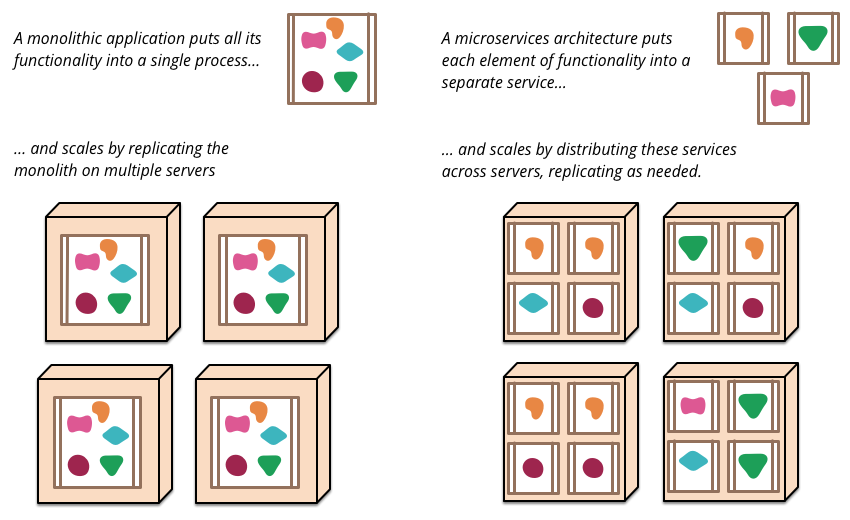
\includegraphics[width=\textwidth, center]{kapitel1/monolith_vs_microservices}
		\caption[Beschreibung für Verzeichnis]{Bildunterschrift}
		\label{img:microprofile}
	\end{figure}
	
	\subsection{Was sind Microservices}
	Lorem ipsum dolor sit amet, consetetur sadipscing elitr, sed diam nonumy eirmod tempor invidunt ut labore et dolore magna aliquyam erat, sed diam voluptua. At vero eos et accusam et justo duo dolores et ea rebum. Stet clita kasd gubergren, no sea takimata sanctus est Lorem ipsum dolor sit amet. Lorem ipsum dolor sit amet, consetetur sadipscing elitr, sed diam nonumy eirmod tempor invidunt ut labore et dolore magna aliquyam erat, sed diam voluptua. At vero eos et accusam et justo duo dolores et ea rebum. Stet clita kasd gubergren, no sea takimata sanctus est Lorem ipsum dolor sit amet \cite{Reese2009}.
	
	\paragraph{Klein und spezialisiert} Lorem ipsum dolor sit amet, consetetur sadipscing elitr, sed diam nonumy eirmod tempor invidunt ut labore et dolore magna aliquyam erat, sed diam voluptua. At vero eos et accusam et justo duo dolores et ea rebum. Stet clita kasd gubergren, no sea takimata sanctus est Lorem ipsum dolor sit amet. Lorem ipsum dolor sit amet, consetetur sadipscing elitr, sed diam nonumy eirmod tempor invidunt ut labore et dolore magna aliquyam erat, sed diam voluptua. At vero eos et accusam et justo duo dolores et ea rebum. Stet clita kasd gubergren, no sea takimata sanctus est Lorem ipsum dolor sit amet.
	
	\paragraph{Eigenständig} Lorem ipsum dolor sit amet, consetetur sadipscing elitr, sed diam nonumy eirmod tempor invidunt ut labore et dolore magna aliquyam erat, sed diam voluptua. At vero eos et accusam et justo duo dolores et ea rebum. Stet clita kasd gubergren, no sea takimata sanctus est Lorem ipsum dolor sit amet. Lorem ipsum dolor sit amet, consetetur sadipscing elitr, sed diam nonumy eirmod tempor invidunt ut labore et dolore magna aliquyam erat, sed diam voluptua. At vero eos et accusam et justo duo dolores et ea rebum. Stet clita kasd gubergren, no sea takimata sanctus est Lorem ipsum dolor sit amet. Verweis auf Anhang \ref{appendix:anhanga} \nameref{appendix:anhanga}
 % Externe Datei einbinden
\chapter{Kapitel 2}
\label{chap:kapitel2}
Eine Abkürzung \ac{cd}, \ac{ci}. Ausgeschrieben \acl{cd}. Verweis zu einem File-Listing \ref{lst:crypter} oder einem Listing im Textfluss \ref{lst:Rggplot} und ein Inline-Listing \lstinline|print("Hello World")|.

\lstinputlisting[language=Java,caption={Ein Listing},label=lst:crypter]{\srcloc/Crypter.java}

\begin{lstlisting}[language=R,caption=Beispielaufruf ldply-Funktion in R, label=lst:Rggplot]
ggplot(data = data, mapping = aes(x=timestamp, y=score) + geom_line()
\end{lstlisting}
			 % Externe Datei einbinden
% ------------------------------------------------------------------

\label{lastpage}

% Neue Seite
\cleardoublepage

% Backmatter mit normalem Zeilenabstand setzen
\singlespacing

% Römische Ziffern für die "Back-Matter", fortlaufend mit "Front-Matter"
\pagenumbering{roman}
%\setcounter{page}{\value{frontmatterpage}}
\setcounter{page}{0}
% Abkürzungsverzeichnis
\addchap{\hsmaabbreviations}
\begin{acronym}[IEEE]
	\acro{ml}[ML]{maschinellen Lernens}
	\acro{automl}[AutoML]{automatisierte maschinelle Lernen}
	
	\acro{tfae}[TFAE]{TaskFocusingOnAutoencoder}
	\acro{ttae}[TTAE]{TaskTransferOnAutoencoder}
	\acro{autottae}[AutoTTAE]{AutoTaskTransferOnAutoencoder}
	
	\acro{nas}[NAS]{Neural Architecture Search}
	\acro{hpo}[HPO]{Hyperparameter-Optimierung}	
	\acro{cae}[CAE]{Convolutional Autoencoder}	
	
	\acro{ssd}[SSD]{Single Shot MultiBox Detector}
	
	\acro{mtl}[MTL]{Multi-Task-Lernen}		
	\acro{miso}[MISO]{Multi-Input Single-Output}	
	\acro{simo}[SIMO]{Single-Input Multi-Output}	
	\acro{mimo}[MIMO]{Multi-Input Multi-Output}	
	

	\acro{sh}[SH]{Successive Halving}	
	
	\acro{iou}[IoU]{Intersection over Union}	
\end{acronym}


% Tabellenverzeichnis erzeugen
\cleardoublepage
\phantomsection
\addcontentsline{toc}{chapter}{\hsmalistoftables}
\listoftables

% Abbildungsverzeichnis erzeugen
\cleardoublepage
\phantomsection
\addcontentsline{toc}{chapter}{\hsmalistoffigures}
\listoffigures

% Listingverzeichnis erzeugen
\cleardoublepage
\phantomsection
\addcontentsline{toc}{chapter}{\hsmalistings}
\lstlistoflistings

% Literaturverzeichnis erzeugen
\begin{flushleft}
\printbibliography
\end{flushleft}

% Index ausgeben. Wenn Sie keinen Index haben, entfernen Sie einfach
% diesen Teil.
%\cleardoublepage
%\phantomsection
%\addcontentsline{toc}{chapter}{\hsmaindex}
%\printindex

% Anhang. Wenn Sie keinen Anhang haben, entfernen Sie einfach
% diesen Teil.
\appendix
\chapter{Ein Anhang}
\label{appendix:anhanga}

Referenz zu Tabelle \ref{table:topbeatmetricssystem}.

\begin{table}[ht]
	\centering
	\begin{tabularx}{\textwidth}{msb}
		\textbf{Bezeichnung} 	& \textbf{Typ} 		& \textbf{Beschreibung} 	\\ \hline 
		load.load1 				& float	  			& The load average over 1 minute.				\\ \rowcolor{Gray}
		load.load5 				& float 			& The load average over 5 minutes.				\\ 
		load.load15				& float 			& The load average over 15 minutes.				\\ \rowcolor{Gray}
		cpu.user				& int	 			& The amount of CPU time spent in user space.  	\\ 
		cpu.user\_p				& float	 			& The percentage of CPU time spent in user space. On multi-core systems, you can have percentages that are greater than 100\%. For example, if 3 cores are at 60\% use, then the cpu.user\_p will be 180\%.	\\ \rowcolor{Gray}
		cpu.system				& int	 			& The amount of CPU time spent in kernel space.	\\ 
		cpu.system\_p			& float	 			& The percentage of CPU time spent in kernel space.	\\ \rowcolor{Gray}
		mem.total				& int	 			& Total memory.								  	\\ 
		mem.used				& int	 			& Used memory.								  	\\ \rowcolor{Gray}
		mem.free				& int	 			& Available memory.							  	\\ 
		mem.used\_p				& float	 			& The percentage of used memory.			
	\end{tabularx}
	\caption{Tabellenunterschrift}
	\label{table:topbeatmetricssystem}
\end{table}

\begin{figure}[h]
	\centering
	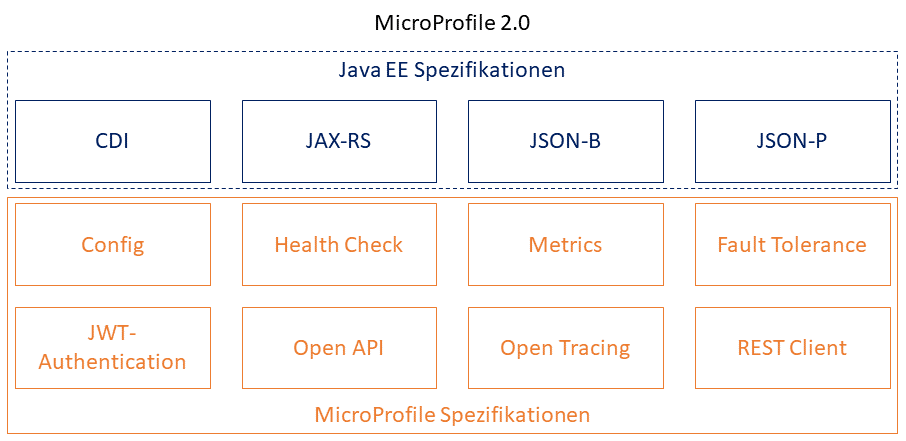
\includegraphics[width=\textwidth, center]{anhanga/microprofile_components}
	\caption[Beschreibung für Verzeichnis2]{Bildunterschrift2}
	\label{img:microprofile_components}
\end{figure}

\end{document}
